\documentclass{article}
\usepackage{ctable,microtype,amsmath,amssymb,graphicx,float}
\usepackage{siunitx}
\usepackage{xkeyval} 
\usepackage{cleveref}
\usepackage[utf8]{inputenc}
\usepackage[danish]{babel}
\usepackage{amsthm}
\setlength\parindent{0pt}
\usepackage{fancyhdr}
\usepackage{dcolumn}
\usepackage[colorlinks,linkcolor=black,citecolor=blue,urlcolor=black]{hyperref}
\usepackage{setspace}
\usepackage[left=25mm, right=25mm, top=25mm, bottom=25mm]{geometry}
\usepackage{minted}
\usepackage{memhfixc}
\usepackage{subfiles}
\usepackage{csquotes}
\usepackage{xcolor}
\definecolor{LightGray}{gray}{0.9}
%\definecolor{DarkGray}{gray}{0.1}
%\pagecolor{DarkGray}
\usemintedstyle{borland}
%New colors defined below
\definecolor{codegreen}{rgb}{0,0.6,0}
\definecolor{codegray}{rgb}{0.5,0.5,0.5}
\definecolor{codepurple}{rgb}{0.58,0,0.82}
\definecolor{backcolour}{rgb}{0.95,0.95,0.92}
\title{Test Driven Development}
\author{Simon Egeberg-201406253}
\usepackage[backend=biber,style=science,sorting=ynt,citestyle=science]{biblatex}
\addbibresource{references.bib}
\usepackage{graphicx}
\begin{document}
\maketitle
\section{Hvorfor TTD?}
Omkring 65\% af prisen på software ligger i at opretholde det software som er udviklet.
\textbf{Code Entropy}:\\
Dette sker fordi kode kan blive ``brittle'' over tid. Det kan være fordi at koden ikke er skalerbar.

\textbf{Isolated Ownership}:\\
Der kan være dele af det som kun en enkelt koder kan dekode og udvikle. 

\textbf{High risk code changes}

\section{Hvad er TDD?}
Inden man ved hvad TDD er, skal man vide hvad en test er. En \textbf{test} er en procedure til at fastslå kvaliteten, performance eller pålideligheden af noget, specielt inden det tages i brug.
Derfor kan en sammensætning af test vide om løsningen rent faktisk ér en løsning. At den smider det rigtige ud, givet inputs, og dens performance er tilstrækkelig. \\
\begin{figure}[H]
	\centering
	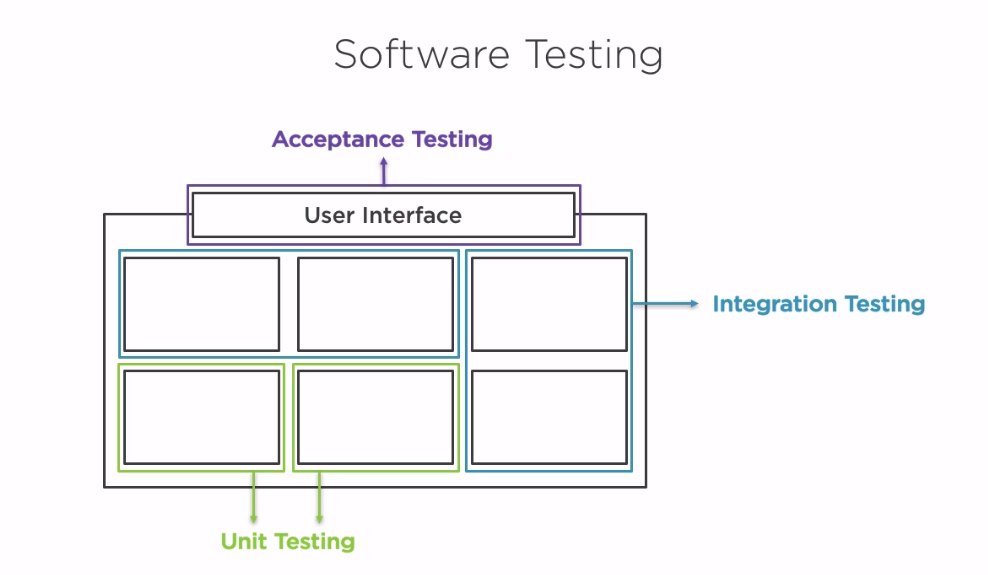
\includegraphics[width = 0.6\textwidth]{softwaretesting.PNG}
\end{figure}

Dette kulminere så i hvad TDD er. Det er en software udviklings process som drejer sig om en meget kort udviklings cyklus som gentages: Krav omskrives til specifikke testcases, også bliver der skrevet software til at bestå de tests.

\begin{figure}[H]
	\centering
	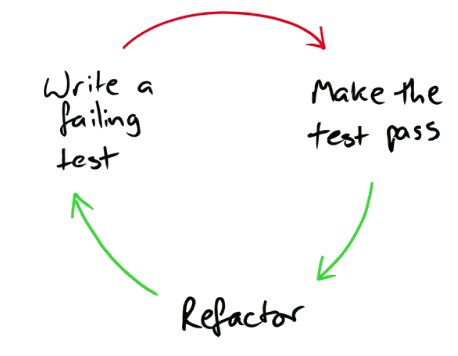
\includegraphics[width = 0.4\textwidth]{redgreen.PNG}
\end{figure}


\section{Værktøjer til TDD}
\subsection{Feature list}
Del projektet op i features. Eksempel: 
\begin{enumerate}
 	\item Feature 1
 	\begin{enumerate}
 		\item Add this
 		\item add that
 	\end{enumerate}
 \end{enumerate} 
Det skal huskes på at en feature list et en levende ting, den kan altid udvides. Der skal bare huskes på: \textbf{RED-GREEN-REFACTOR}

\begin{figure}[H]
	\centering
	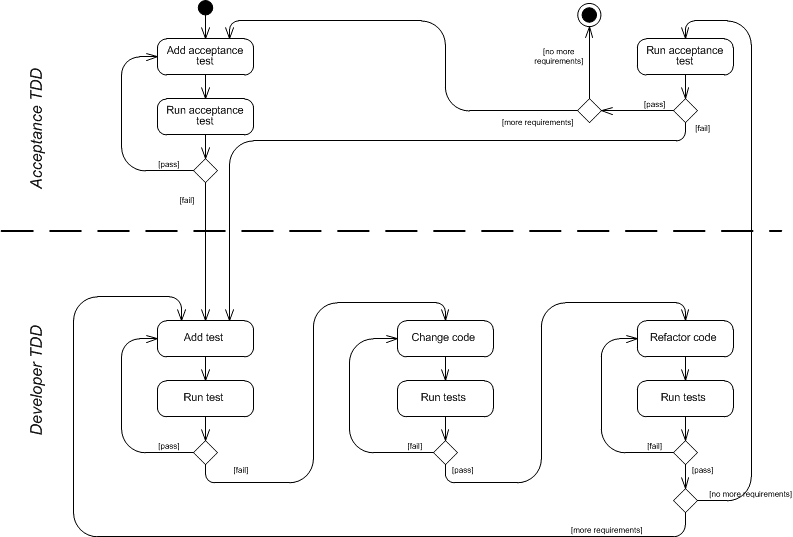
\includegraphics[width = \textwidth]{Billede1.png}
\end{figure}
\end{document}